%%%%%%%%%%%%%%%%%%%%%%%%%%%%%%%%%%%%%%%%%
% Programming/Coding Assignment
% LaTeX Template
%
% This template has been downloaded from:
% http://www.latextemplates.com
%
% Original author:
% Ted Pavlic (http://www.tedpavlic.com)
%
% Note:
% The \lipsum[#] commands throughout this template generate dummy text
% to fill the template out. These commands should all be removed when 
% writing assignment content.
%
% This template uses a Perl script as an example snippet of code, most other
% languages are also usable. Configure them in the "CODE INCLUSION 
% CONFIGURATION" section.
%
%%%%%%%%%%%%%%%%%%%%%%%%%%%%%%%%%%%%%%%%%

%----------------------------------------------------------------------------------------
%	PACKAGES AND OTHER DOCUMENT CONFIGURATIONS
%----------------------------------------------------------------------------------------

\documentclass{article}

\usepackage{fancyhdr} % Required for custom headers
\usepackage{lastpage} % Required to determine the last page for the footer
\usepackage{extramarks} % Required for headers and footers
\usepackage[usenames,dvipsnames]{color} % Required for custom colors
\usepackage{graphicx} % Required to insert images
\usepackage{subcaption}
\usepackage{listings} % Required for insertion of code
\usepackage{courier} % Required for the courier font
\usepackage{amsmath}
\usepackage{framed}

% Margins
\topmargin=-0.45in
\evensidemargin=0in
\oddsidemargin=0in
\textwidth=6.5in
\textheight=9.0in
\headsep=0.25in

\linespread{1.1} % Line spacing

% Set up the header and footer
\pagestyle{fancy}
\lhead{\hmwkAuthorName} % Top left header
\chead{\hmwkClass\ (\hmwkClassTime): \hmwkTitle} % Top center head
%\rhead{\firstxmark} % Top right header
\lfoot{\lastxmark} % Bottom left footer
\cfoot{} % Bottom center footer
\rfoot{Page\ \thepage\ of\ \protect\pageref{LastPage}} % Bottom right footer
\renewcommand\headrulewidth{0.4pt} % Size of the header rule
\renewcommand\footrulewidth{0.4pt} % Size of the footer rule

\setlength\parindent{0pt} % Removes all indentation from paragraphs

%----------------------------------------------------------------------------------------
%	CODE INCLUSION CONFIGURATION
%----------------------------------------------------------------------------------------

\definecolor{mygreen}{rgb}{0,0.6,0}
\definecolor{mygray}{rgb}{0.5,0.5,0.5}
\definecolor{mymauve}{rgb}{0.58,0,0.82}

\lstset{ %
  backgroundcolor=\color{white},   % choose the background color
  basicstyle=\footnotesize,        % size of fonts used for the code
  breaklines=true,                 % automatic line breaking only at whitespace
  captionpos=b,                    % sets the caption-position to bottom
  commentstyle=\color{mygreen},    % comment style
  escapeinside={\%*}{*)},          % if you want to add LaTeX within your code
  keywordstyle=\color{blue},       % keyword style
  stringstyle=\color{mymauve},     % string literal style
}

%----------------------------------------------------------------------------------------
%	DOCUMENT STRUCTURE COMMANDS
%	Skip this unless you know what you're doing
%----------------------------------------------------------------------------------------

% Header and footer for when a page split occurs within a problem environment
\newcommand{\enterProblemHeader}[1]{
%\nobreak\extramarks{#1}{#1 continued on next page\ldots}\nobreak
%\nobreak\extramarks{#1 (continued)}{#1 continued on next page\ldots}\nobreak
}

% Header and footer for when a page split occurs between problem environments
\newcommand{\exitProblemHeader}[1]{
%\nobreak\extramarks{#1 (continued)}{#1 continued on next page\ldots}\nobreak
%\nobreak\extramarks{#1}{}\nobreak
}

\setcounter{secnumdepth}{0} % Removes default section numbers
\newcounter{homeworkProblemCounter} % Creates a counter to keep track of the number of problems
\setcounter{homeworkProblemCounter}{0}

\newcommand{\homeworkProblemName}{}
\newenvironment{homeworkProblem}[1][Problem \arabic{homeworkProblemCounter}]{ % Makes a new environment called homeworkProblem which takes 1 argument (custom name) but the default is "Problem #"
\stepcounter{homeworkProblemCounter} % Increase counter for number of problems
\renewcommand{\homeworkProblemName}{#1} % Assign \homeworkProblemName the name of the problem
\section{\homeworkProblemName} % Make a section in the document with the custom problem count
\enterProblemHeader{\homeworkProblemName} % Header and footer within the environment
}{
\exitProblemHeader{\homeworkProblemName} % Header and footer after the environment
}

\newcommand{\problemAnswer}[1]{ % Defines the problem answer command with the content as the only argument
\noindent\framebox[\columnwidth][c]{\begin{minipage}{0.98\columnwidth}#1\end{minipage}} % Makes the box around the problem answer and puts the content inside
}

\newcommand{\homeworkSectionName}{}
\newenvironment{homeworkSection}[1]{ % New environment for sections within homework problems, takes 1 argument - the name of the section
\renewcommand{\homeworkSectionName}{#1} % Assign \homeworkSectionName to the name of the section from the environment argument
\subsection{\homeworkSectionName} % Make a subsection with the custom name of the subsection
\enterProblemHeader{\homeworkProblemName\ [\homeworkSectionName]} % Header and footer within the environment
}{
\enterProblemHeader{\homeworkProblemName} % Header and footer after the environment
}

%----------------------------------------------------------------------------------------
%	NAME AND CLASS SECTION
%----------------------------------------------------------------------------------------

\newcommand{\hmwkTitle}{Assignment 4} % Assignment title
\newcommand{\hmwkDueDate}{Monday, Apr. 2, 2018} % Due date
\newcommand{\hmwkClass}{CSC411} % Course/class
\newcommand{\hmwkClassTime}{LEC 5101/0101} % Class/lecture time
\newcommand{\hmwkAuthorName}{Zhongtian Ouyang/Yihao Ni} % Your name

%----------------------------------------------------------------------------------------
%	TITLE PAGE
%----------------------------------------------------------------------------------------

\title{
\vspace{2in}
\textmd{\textbf{\hmwkClass:\ \hmwkTitle}}\\
\normalsize\vspace{0.1in}\small{Due\ on\ \hmwkDueDate}\\
\vspace{0.1in}
\vspace{3in}
}

\author{\textbf{\hmwkAuthorName}}
\date{} % Insert date here if you want it to appear below your name

%----------------------------------------------------------------------------------------

\begin{document}

\maketitle
\clearpage
%----------------------------------------------------------------------------------------
%	PROBLEM 1
%----------------------------------------------------------------------------------------

% To have just one problem per page, simply put a \clearpage after each problem

\begin{homeworkProblem}

\noindent \textit{Environment}\\
The grid is a three by three matrix, where every spot is '.' when it is empty, 'x' for player one and 'o' for player two. The attribute turn is 1 when player one is playing, and 2 when player two is playing. The attribute done is True in two cases, either the game is in a win state, or all of the spots are filled.\\
Following is the output of a game of tic-tac-toe against myself.
\begin{framed}
\begin{lstlisting}[language=python]
>>> from tictactoe import Environment
>>> ttt = Environment()
>>> ttt.step(4)
(array([0, 0, 0, 0, 1, 0, 0, 0, 0]), 'valid', False)
>>> ttt.step(0)
(array([2, 0, 0, 0, 1, 0, 0, 0, 0]), 'valid', False)
>>> ttt.step(1)
(array([2, 1, 0, 0, 1, 0, 0, 0, 0]), 'valid', False)
>>> ttt.step(3)
(array([2, 1, 0, 2, 1, 0, 0, 0, 0]), 'valid', False)
>>> ttt.step(7)
(array([2, 1, 0, 2, 1, 0, 0, 1, 0]), 'win', True)
>>> ttt.render()
ox.
ox.
.x.
====
\end{lstlisting}
\end{framed}

\end{homeworkProblem}
\clearpage
%----------------------------------------------------------------------------------------
%	PROBLEM 2
%----------------------------------------------------------------------------------------
\begin{homeworkProblem}
\noindent \textit{Policy}\\
 Part a) 
\begin{framed}
\begin{lstlisting}[language=python]
class Policy(nn.Module):
    """
    The Tic-Tac-Toe Policy
    """
    def __init__(self, input_size=27, hidden_size=64, output_size=9):
        super(Policy, self).__init__()
        self.net = torch.nn.Sequential(
            torch.nn.Linear(input_size, hidden_size),
            torch.nn.ReLU(),
            torch.nn.Linear(hidden_size, output_size),
            torch.nn.Softmax(dim=1)
        )

    def forward(self, x):
        return self.net(x)
\end{lstlisting}
\end{framed}

Part b)\\
With a input of 9-dimensional state, the 27-dimensional state is generated with the following two lines.
\begin{framed}
\begin{lstlisting}[language=python]
state = torch.from_numpy(state).long().unsqueeze(0)
state = torch.zeros(3,9).scatter_(0,state,1).view(1,27)
\end{lstlisting}
\end{framed}
Run this two lines with input 
\begin{framed}
\begin{lstlisting}[language=python]
state = np.array([1, 0, 2, 0, 1, 1, 0, 0, 2])
\end{lstlisting}
\end{framed}
After execute the two lines, we got
\begin{framed}
\begin{lstlisting}[language=python]
Columns 0 to 12 
    0     1     0     1     0     0     1     1     0     1     0     0     0
Columns 13 to 25 
    1     1     0     0     0     0     0     1     0     0     0     0     0
Columns 26 to 26 
    1

\end{lstlisting}
\end{framed}
So the output implies that the first 9 columns indicate whether an entry is empty, the second 9 columns indicate whether an entry is ``x'', the third 9 columns indicate whether an entry is ``o''.\\
\\
Part c)\\
The 9-dimensional vector represents the preference/probability of playing each positions. So the first dimension is the preference/probability of making action 1, the second dimension is the preference/probability of making action 2, etc.  Our policy is stochastic.
\end{homeworkProblem}
\clearpage

%----------------------------------------------------------------------------------------
%	PROBLEM 3
%----------------------------------------------------------------------------------------

\begin{homeworkProblem}
\noindent \textit{Compute the gradient}
Part a)
\begin{framed}
\begin{lstlisting}[language=python]
def compute_returns(rewards, gamma=1.0):
    """
    Compute returns for each time step, given the rewards
      @param rewards: list of floats, where rewards[t] is the reward
                      obtained at time step t
      @param gamma: the discount factor
      @returns list of floats representing the episode's returns
          G_t = r_t + \gamma r_{t+1} + \gamma^2 r_{t+2} + ...

    >>> compute_returns([0,0,0,1], 1.0)
    [1.0, 1.0, 1.0, 1.0]
    >>> compute_returns([0,0,0,1], 0.9)
    [0.7290000000000001, 0.81, 0.9, 1.0]
    >>> compute_returns([0,-0.5,5,0.5,-10], 0.9)
    [-2.5965000000000003, -2.8850000000000002, -2.6500000000000004, -8.5, -10.0]
    """
    max_t = len(rewards)
    result = [0] * max_t
    for i in range(max_t):
        for j in range(i, max_t):
            result[i] += rewards[j] * (gamma**(j-i))
    return result
\end{lstlisting}
\end{framed}
Part b)\\
We can't update weights in the middle of an episode because the policy is for playing the whole game, not a single step. So if we change weights during a game, we can't assess how good this policy is. And the expected total reward won't be correct. 

\end{homeworkProblem}
\clearpage
%----------------------------------------------------------------------------------------
%	PROBLEM 4
%----------------------------------------------------------------------------------------

\begin{homeworkProblem}
\noindent \textit{Choosing rewards}\\
Part a)\\
\begin{framed}
\begin{lstlisting}[language=python]
def get_reward(status):
    """Returns a numeric given an environment status."""
    return {
            Environment.STATUS_VALID_MOVE  : 0, # TODO
            Environment.STATUS_INVALID_MOVE: -15,
            Environment.STATUS_WIN         : 10,
            Environment.STATUS_TIE         : -1,
            Environment.STATUS_LOSE        : -10
    }[status]
\end{lstlisting}
\end{framed}

Part b)\\
Valid move is zero, win is positive and all the others are negative. Valid move is not encouraged or discouraged so it is zero. We do not want any invalid moves, even if we are losing, so it is negative and the magnitude is larger then win. The value of tie does not matter much as long as it is between win and lose. However, the goal is to win so we give tie a negative value. Lose is of course negative and as mentioned before, its magnitude should be smaller than invalid move.


\end{homeworkProblem}
\clearpage

%----------------------------------------------------------------------------------------
%	PROBLEM 5
%----------------------------------------------------------------------------------------

\begin{homeworkProblem}
\noindent \textit{Training the policy}\\
Part a)\\
Following is the training curve with the rewards chosen from problem 4. The only hyperparameter to change is the value for gamma. We tried values 0.7, 0.8, 0.9 and 1.0. 0.8 gives the best win rate against random.
\begin{figure}[!ht]
\centering
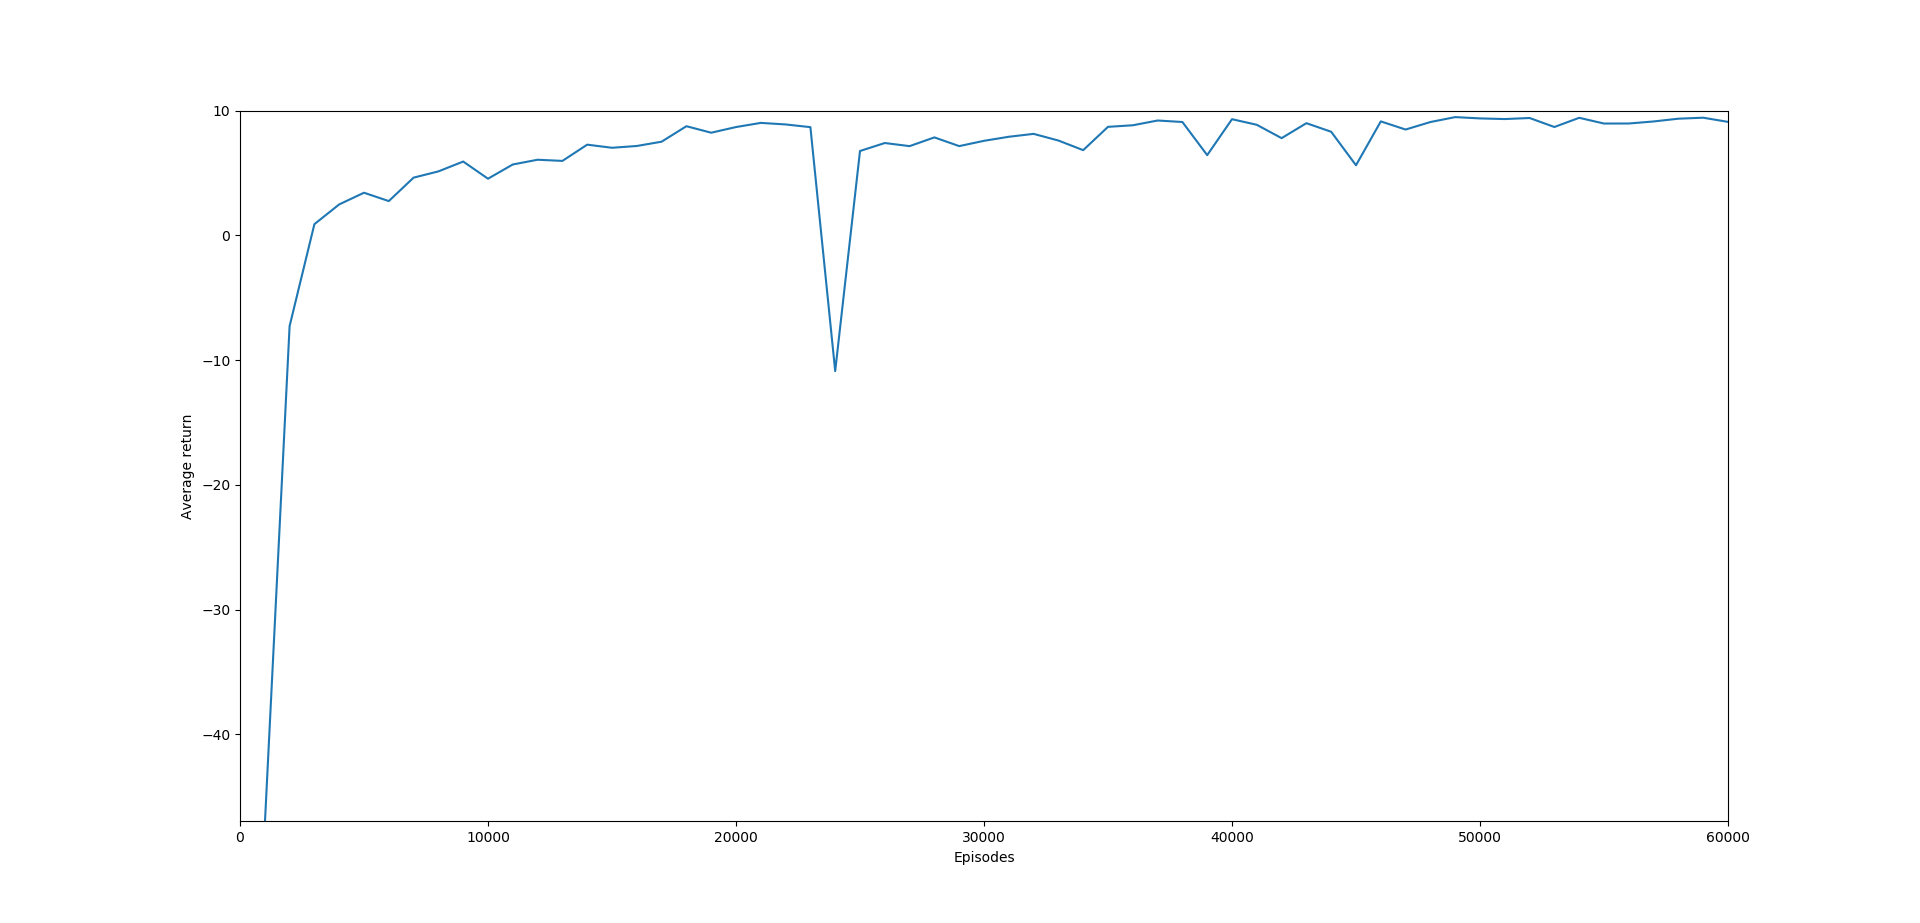
\includegraphics[width=0.7\linewidth]{p5a.png}
\caption{training curve}
\label{fig:p5a}
\end{figure}
\\
Part b)\\
To find out what is the best number of hidden units, I train the policy with 54,64,128,256 hidden units. Then I find out their winrates on playing 400 games with a random player2 using the weights at 1000, 2000, 3000, ....., 60000 episodes. The one with the best winrate what we want. In my case, it is the policy with 64 hidden units at episode 49000. The win rate is 97.75 \%.\\
\\
Part c) \\
The following graph is obtained by playing 400 games with a random player 2 using the best policy with weights from episode 1000, 2000, 3000, ...., 60000. The total number of invalid moves chose by our policy divided by 400 would get us the below values. From the graph, we can see that our policy learn to not made invalid moves at around 5000 episodes. After that, the rate is just oscillating between 0 and 0.25 invalid moves per game. As a reference, in the  previous part, at 49000, our best performance episode, only 1 invalid move is made throughout the 400 games.
\begin{figure}[!ht]
\centering
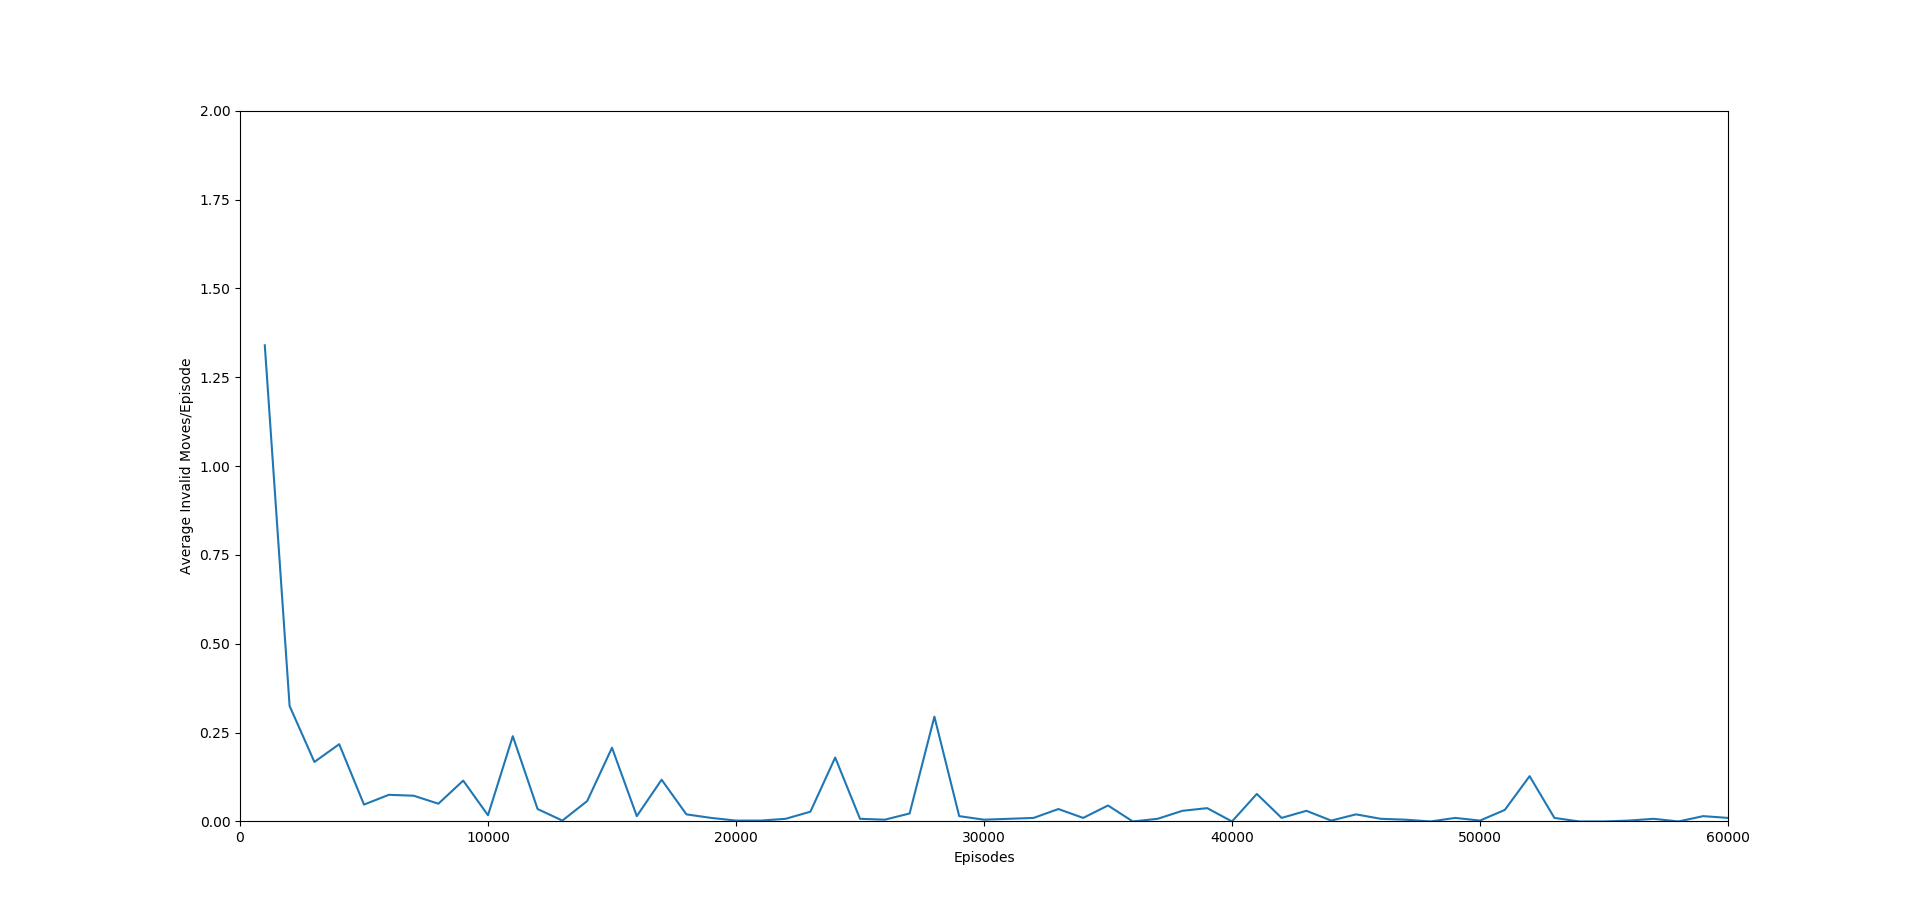
\includegraphics[width=0.7\linewidth]{p5c.png}
\caption{Average invalid moves per game}
\label{fig:p5c}
\end{figure}
\\
\\
Part d)\\
Following is the performance of our learned policy against random (output format is modified to better display the result):
\begin{framed}
\begin{lstlisting}[language=python]
===============================Part 5d==============================
Use weights from episode 49000
100 games played:
Win: 92 Percentage: 0.92
Lose: 1 Percentage: 0.01
Tie: 7 Percentage: 0.07
0 invalid actions are made

===== Game1 =====
..x   ..x   ..x   ..x   ..x
...   o..   o.x   o.x   o.x
...   ...   ...   .o.   .ox
Learned policy wins against random!

===== Game2 =====
..x   .ox   .ox   .ox   .ox
...   ...   ...   .o.   .ox
...   ...   ..x   ..x   ..x
Learned policy wins against random!

===== Game3 =====
..x   .ox   .ox   .ox   .ox   .ox   xox
...   ...   ...   ..o   .xo   .xo   .xo
...   ...   ..x   ..x   ..x   .ox   .ox
Learned policy wins against random!

===== Game4 =====
..x   ..x   x.x   x.x   xxx
...   ...   ...   ...   ...
...   ..o   ..o   .oo   .oo
Learned policy wins against random!

===== Game5 =====
..x   ..x   ..x   .ox   .ox
...   ...   ..x   ..x   ..x
...   .o.   .o.   .o.   .ox
Learned policy wins against random!
\end{lstlisting}
\end{framed}
\end{homeworkProblem}
The policy learned to place the first cross at the right-corner position, and tries to win the game by filling the right colomn. It does not make any invalid move and if there is a chance to win, it wins. However, it may not know how to not lose, ie. to block the opponent to win.
\clearpage
%----------------------------------------------------------------------------------------
%	PROBLEM 6
%----------------------------------------------------------------------------------------
\begin{homeworkProblem}
\noindent \textit{Win rate throughout training}\\
From the graph below, we could see that thoughout training, even though the win rate is not stable, the overall trend is increasing, accompanied by the decreasing of both tie rate and loss rate. At around 40000 episode, the performance start to stablize.
\begin{figure}[!ht]
\centering
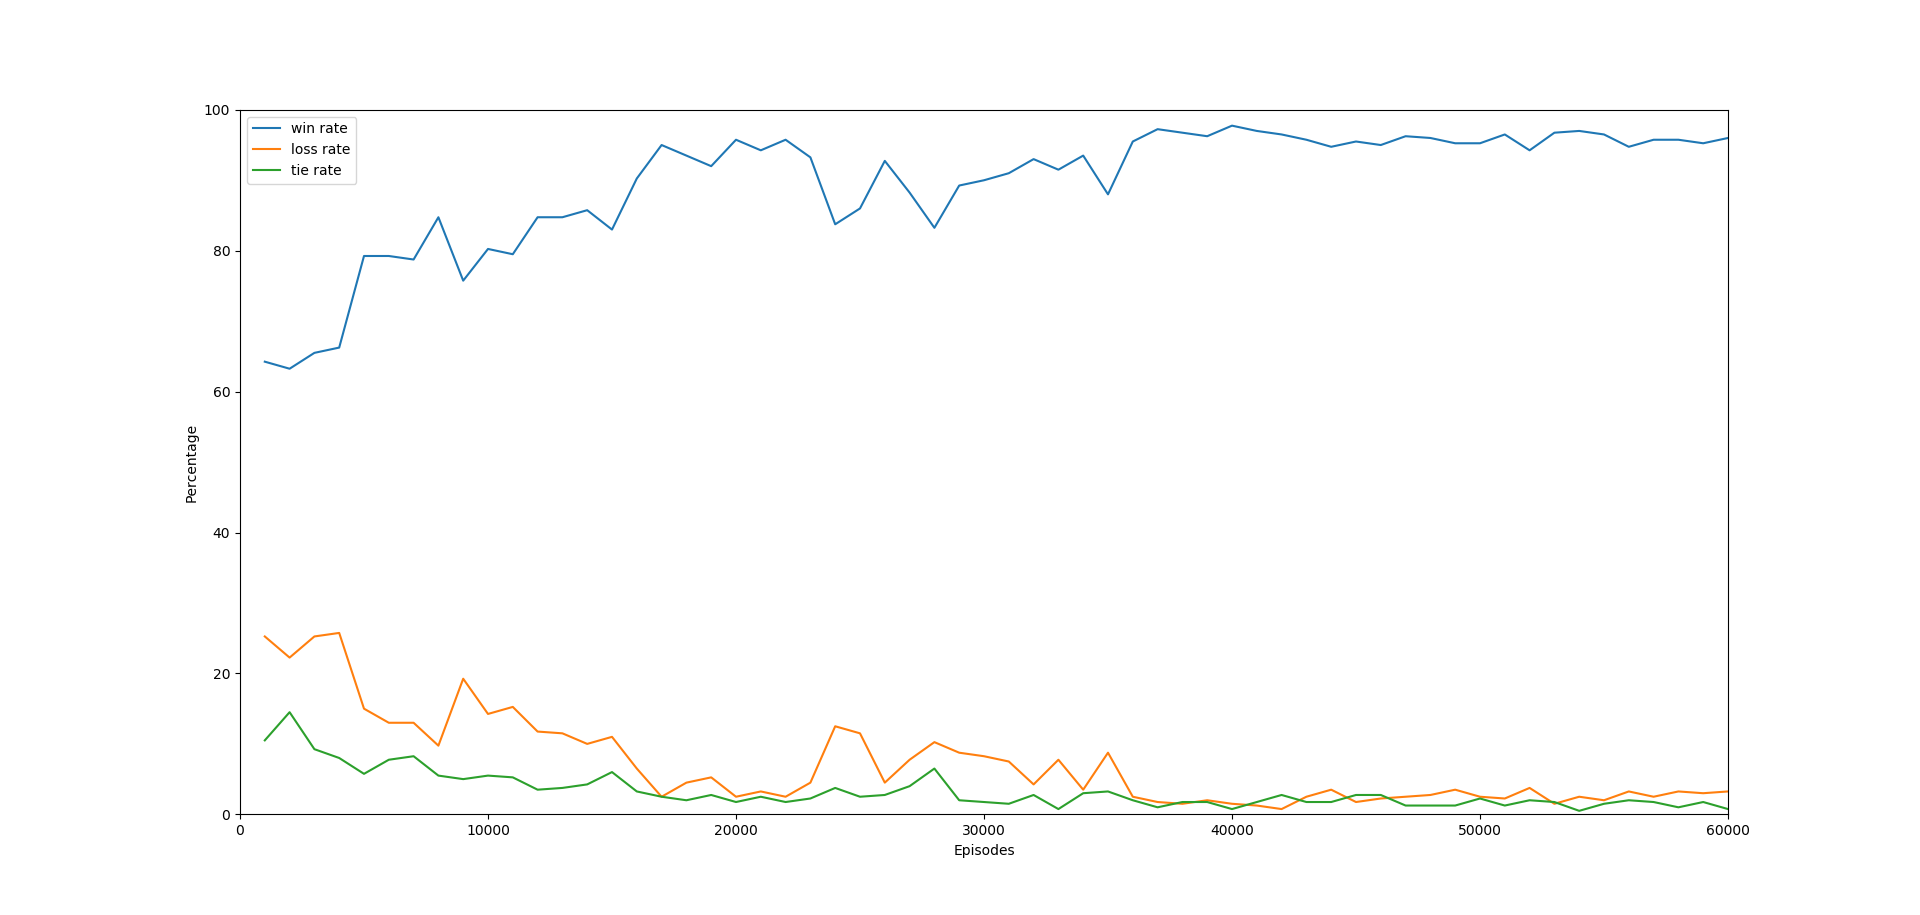
\includegraphics[width=1\linewidth]{p6.png}
\caption{Win rate}
\label{fig:p7}
\end{figure}
\end{homeworkProblem}
\clearpage
%----------------------------------------------------------------------------------------
%	PROBLEM 7
%----------------------------------------------------------------------------------------
\begin{homeworkProblem}
\noindent \textit{First move distribution}
\begin{framed}
\begin{lstlisting}[language=python]
Distribution of the first step from policy with 64 hidden units at episode 49000
Probability playing position 0: 0.00 %
Probability playing position 1: 0.00 %
Probability playing position 2: 1.00 %
Probability playing position 3: 0.00 %
Probability playing position 4: 0.00 %
Probability playing position 5: 0.00 %
Probability playing position 6: 0.00 %
Probability playing position 7: 0.00 %
Probability playing position 8: 0.00 %
\end{lstlisting}
\end{framed}
I first thought this is unreasonable as we instinctly feels the center(position 4) is the best first move to made. However, with some research online about the tictactoe game and I found out that that placing the first move at one of the corners is at least as good as, if not better than, placing the first move at the center. Since position 2 is the top right corner, this first move is reasonable. Especially when facing an random opponent. When this first move is at corner, the only way that player 2 can tie the game, assume player one plays perfectly, is put the first move at center and second move in one of following positions: 1,3,5,7. The chance for a random player 2 for doing that is 1/8 * 2/3 = 1/12.\\
reference: https://www.quora.com/Is-there-a-way-to-never-lose-at-Tic-Tac-Toe\\
\\
Below is a graph showing how the distribution changed throughout training. We can see that for the first 10000 episodes, the policy is not very sure what to do. After that it starts to oscillate between position 0, 2, 5. 0 and 2 are both a corner position as stated above, while 5 is a as good selection. And this is shown by the fact that postition 5 is dominant for less and less episodes as the policy evolve. And from episodes 40000 and onward, it decides position 2 is the best first move and keeps doing that.
\begin{figure}[!ht]
\centering
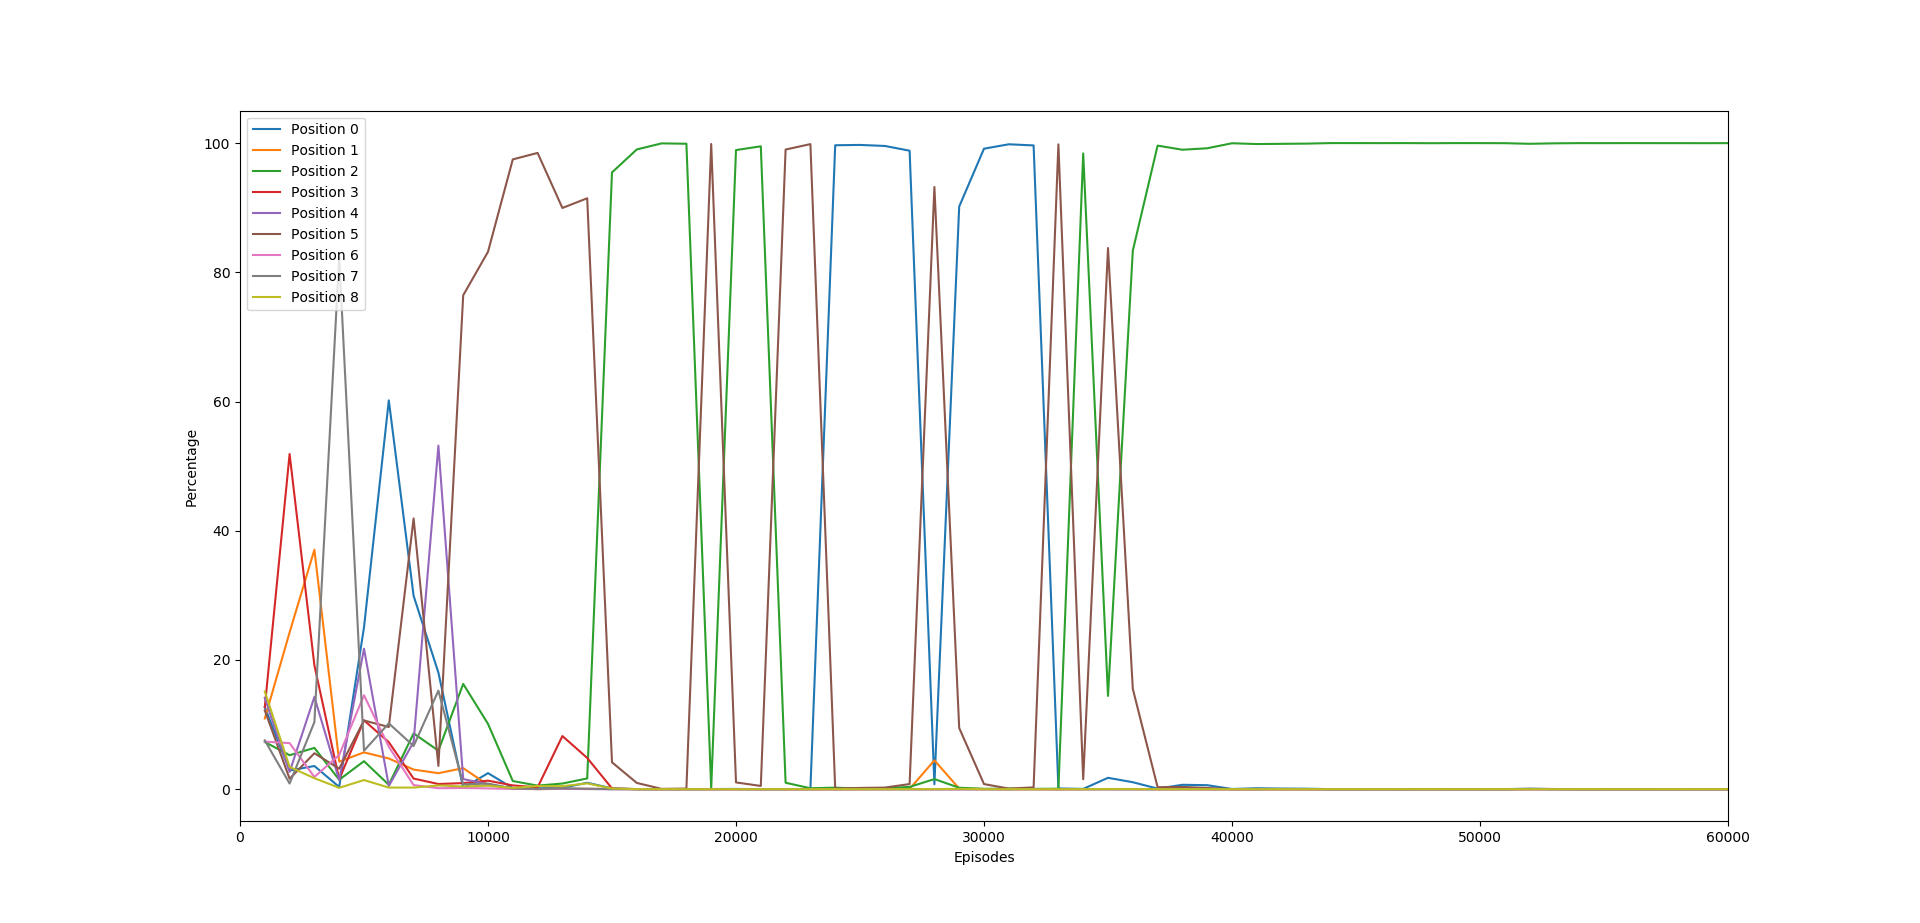
\includegraphics[width=1\linewidth]{p7.png}
\caption{First move distribution}
\label{fig:p7}
\end{figure}
\end{homeworkProblem}
\clearpage
%----------------------------------------------------------------------------------------
%	PROBLEM 8
%----------------------------------------------------------------------------------------
\begin{homeworkProblem}
\noindent \textit{Limitation}\\
The limitation of our learned policy is that it doesn't learn how to stop opponent from winning. Since out policy is trained facing an random policy, it doesn't expect the opponent to deliberately trying to win. And so it doesn't develop a stratage that would effectively and actively prevent opponent from winning
\end{homeworkProblem}
\clearpage
%----------------------------------------------------------------------------------------

\end{document}
